\documentclass{beamer}

\usetheme[secheader]{Boadilla}

\usepackage{xecolor}
\usepackage{datetime}

\newdateformat{minimaldate}{%
  \shortmonthname[\THEMONTH] \THEYEAR}

\author[Elahe Dastan]{%
  Elahe Dastan\hfill
  9631025\\
  \texttt{elahe.dstn@gmail.com}
}
\title{Traffic Flow Prediction With Big Data}
\subtitle{A Deep Learning Approach}
\institute[AUT]{Machine Learning\\Amirkabir University of Technology}
\date{\minimaldate\today}

\begin{document}

\begin{frame}
  \titlepage{}
\end{frame}
\begin{frame}
  \frametitle{Outline}
  \tableofcontents{}
\end{frame}

\section{Introduction}

\begin{frame}
  \frametitle{Goal}
	\begin{columns}
		\column{.5\textwidth}
		\par
		a service which asks the user to select two points as source and destination on the map and
		service can inform the user how long it takes him/her to travel from source to destination.
		\column{.5\textwidth}
		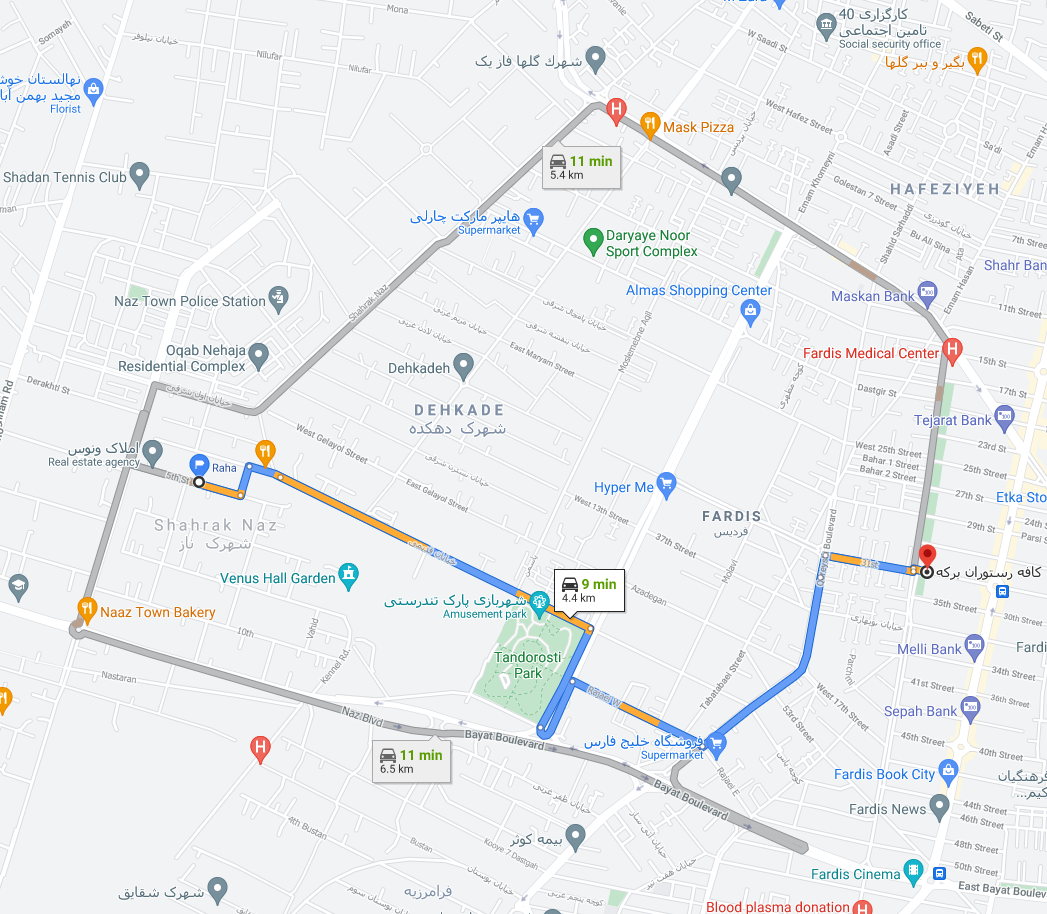
\includegraphics[height=0.5\textheight]{./img/intro.png}
	\end{columns}
\end{frame}
\begin{frame}
  \frametitle{This is done before}
	\begin{columns}
		\column{.25\textwidth}
		
\includegraphics[height=0.5\textheight]{./img/google-maps.png}
		\textbf{Google Maps}\\
		\textit{Google}
		\column{.25\textwidth}
		
\includegraphics[height=0.5\textheight]{./img/waze.png}
		\textbf{Waze}\\
		\textit{Google}
		\column{.25\textwidth}
		
\includegraphics[height=0.5\textheight]{./img/balad.png}
		\textbf{Balad}\\
		\textit{Naghshe Pardazan Ertabatat Novin}
		\column{.25\textwidth}
		
\includegraphics[height=0.5\textheight]{./img/neshan.png}
		\textbf{Neshan}\\
		\textit{Neshan Maps Platform}
	\end{columns}
\end{frame}

\end{document}
